\documentclass[a4paper,12pt]{article}
\usepackage[utf8]{inputenc}
\usepackage{graphicx}
\usepackage{fancyhdr}
\usepackage{amsmath}
\usepackage{adjustbox}
\usepackage{mathtools}
\usepackage{float}
\usepackage[spanish]{babel} 
\usepackage{lastpage}
\usepackage{amssymb} % Para símbolos matemáticos adicionales
\usepackage{cleveref}
\usepackage[none]{hyphenat}
\usepackage{array}

\usepackage{multirow}
\usepackage{textcomp}
\usepackage[left=2.5cm, right=2.5cm, top=3cm, bottom=3cm]{geometry}

\graphicspath{{Imagenes/}}

% Encabezado y pie de página
\pagestyle{fancy}
\fancyhf{}
\setlength{\headheight}{30 pt}
\renewcommand{\headrulewidth}{0.2pt}
\fancyhead[R]{\begin{tabular}{@{}l@{}}
\includegraphics[scale=0.4]{escudo.PNG}\end{tabular}}
\fancyhead[L]{\begin{tabular}{@{}c@{}} \textbf{Robótica I - Año: 2024} \\ Trabajo Práctico 2: Herramientas Matemáticas \end{tabular}}


\fancyfoot[R]{\thepage}
\fancyfoot[C]{\begin{tabular}{@{}c@{}}\textbf{BORQUEZ PEREZ Juan Manuel}\\ \textbf{Legajo 13567}\end{tabular}}
\renewcommand{\footrulewidth}{0.2pt}

\begin{document}

\begin{titlepage}
    \centering
    \vspace*{5cm}
    {\Huge\bfseries Informe de Trabajo Práctico N°2}\\
    \vspace{0.2cm}
    {\Large \textbf{Herramientas Matemáticas}}\\
    \vspace{0.5cm}
    {\Large Robótica I}\\
    \vspace{0.5 cm}
    {\Large Ingeniería en Mecatrónica}\\
    \vspace{0.2 cm}
    {\Large Facultad de Ingeniería - UNCUYO}\\
    \vspace{1.5cm}
    Alumno: Juan Manuel BORQUEZ PEREZ\\
    Legajo: 13567\\
    \vfill
    {\begin{tabular}{@{}c@{}}
\includegraphics[scale=0.4]{escudo.PNG}\end{tabular}}\hspace{10pt}
    %Año 2023
\end{titlepage}

\section{Ejercicio 1.}
Grafique el sistema \textbf{\{M\}} respecto de \textbf{\{O\}} para cada una de las siguientes matrices
de rotación:

Se utiliza la función $\mathbf{trplot}$ del \textbf{Robotic Toolbox} para obtener las gráficas.

Se utiliza la función $\mathbf{tr2eul}$ para obtener los \textbf{ángulos de Euler} (roll, pitch, yaw).

\subsection{Inciso a}
\begin{equation*}
    \prescript{O}{}{Rot_M} = 
    \begin{bmatrix}
        0.500 & -0.866\\
        0.866 & 0.500
    \end{bmatrix}
\end{equation*}

\begin{figure}[H]
    \centering
    \begin{adjustbox}{scale = 0.85, max width=\columnwidth}
        \framebox{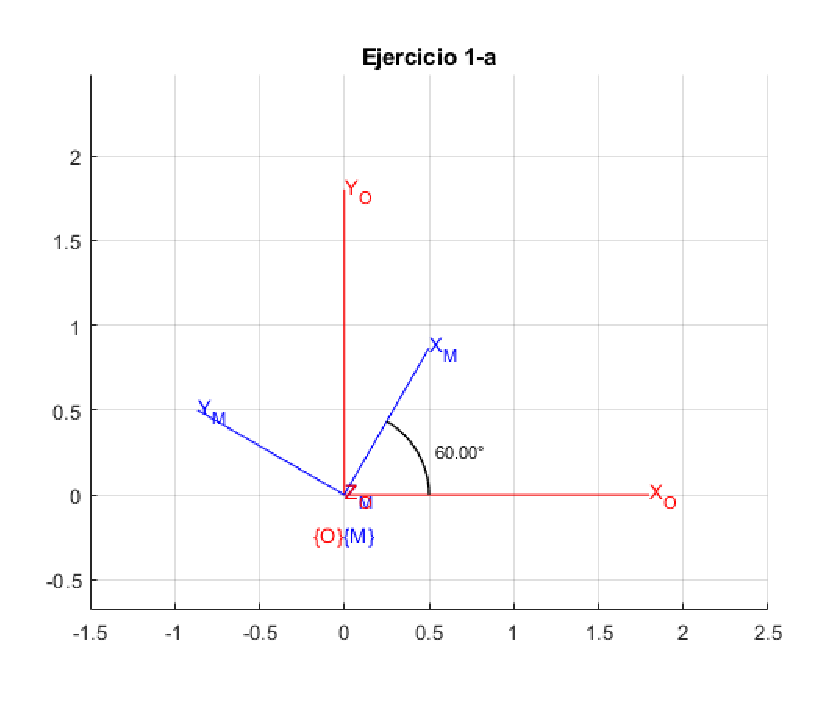
\includegraphics{1-Ejercicio_1_a.pdf}}
    \end{adjustbox}
    \caption{Sistema O y Sistema M superpuestos con indicación de ángulo de rotación.}
\end{figure}

\subsection{Inciso b}
\begin{equation*}
    \prescript{O}{}{Rot_M} = 
    \begin{bmatrix}
        0  &  0  & 1 \\
        -1 &  0  & 0 \\
        0  & -1  & 0
    \end{bmatrix}
\end{equation*}

Para este caso los ángulos de rotación pueden ser:
\begin{align*}
    roll  &=   0^\circ\\
    pitch &=  90^\circ\\
    yaw   &= -90^\circ
\end{align*}

Otra posibilidad es:
\begin{align*}
    roll  &= -90^\circ\\
    pitch &=  90^\circ\\
    yaw   &=   0^\circ
\end{align*}
    
\begin{figure}[H]
    \centering
    \begin{adjustbox}{scale = 0.85, max width=\columnwidth}
        \framebox{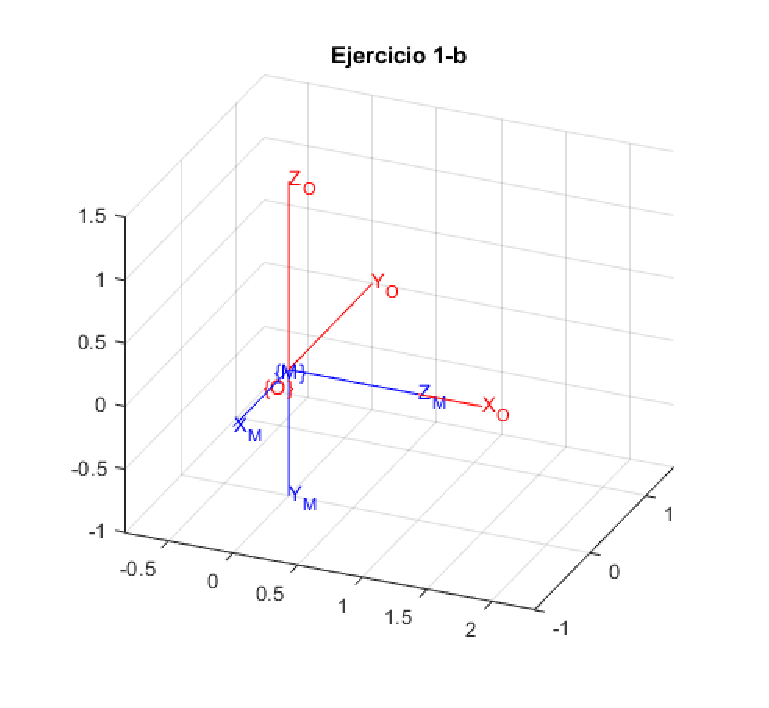
\includegraphics{2-Ejercicio_1_b.pdf}}
    \end{adjustbox}
    \caption{Sistema O y Sistema M superpuestos}
\end{figure}

\subsection{Inciso c}
\begin{equation*}
    \prescript{M}{}{Rot_O} = 
    \begin{bmatrix}
        0.500  &  -0.750  & -0.433 \\
        0.866  &  0.433   & 0.250 \\
        0      & -0.500   & 0.866
    \end{bmatrix}
\end{equation*}

La matriz $\prescript{O}{}{Rot_M}$, que es la inversa de la matriz $\prescript{M}{}{Rot_O}$ por corresponder a la transformación inversa,
se obtiene simplemente transponiendo la matriz $\prescript{M}{}{Rot_O}$. Esto dado que las matrices de rotación y por lo tanto las matrices de 
transformación homogénea correspondientes son ortogonales (en particular ortonormales).

\begin{equation*}
    \prescript{O}{}{Rot_M} = 
    \begin{bmatrix}
        0.500  &  0.866   & 0      \\
        -0.750 &  0.433   & -0.500 \\
        -0.433 &  0.250   & 0.866
    \end{bmatrix}
\end{equation*}

Para este caso los ángulos de rotación son:
\begin{align*}
    roll  &= -90^\circ\\
    pitch &=  30^\circ\\
    yaw   &=  30^\circ
\end{align*}
    
\begin{figure}[H]
    \centering
    \begin{adjustbox}{scale = 0.85, max width=\columnwidth}
        \framebox{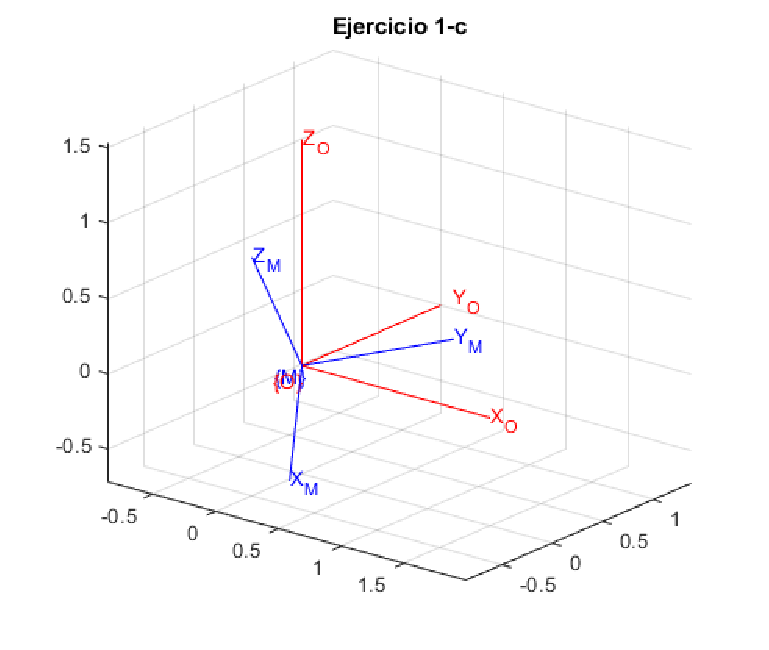
\includegraphics{3-Ejercicio_1_c.pdf}}
    \end{adjustbox}
    \caption{Sistema O y Sistema M superpuestos}
\end{figure}


\section{Ejercicio 2 (obligatorio).}

Exprese cada uno de los siguientes vectores en el sistema de referencia \textbf{\{O\}} sabiendo que sus coordenadas son respecto al sistema \textbf{\{M\}},
el cual sufrió la rotación indicada. Realice un gráfico donde se aprecie el vector y sus coordenadas en ambos 
sistemas.

Se utilizan las funciones \textbf{trot2, trotx, troty, trotz} para obtener las matrices de transformación
homogénea $\prescript{O}{}{T_M}$.

\begin{equation}
    \prescript{O}{}{a} = \prescript{O}{}{T_M}\prescript{M}{}{a}
    \label{transformacion}
\end{equation}


\subsection{Inciso a}
\begin{equation*}
    \prescript{M}{}{a} = 
    \begin{bmatrix}
        1 & 0.5
    \end{bmatrix}
    \rightarrow \{M\} \, \text{rotó} \,  -17^\circ \, \text{en}\, Z_O
\end{equation*}

\begin{equation*}
    \prescript{O}{}{a} = 
    \begin{bmatrix}
        1.1025 & 0.1858
    \end{bmatrix}
\end{equation*}

\begin{figure}[H]
    \centering
    \begin{adjustbox}{scale = 0.85, max width=\columnwidth}
        \framebox{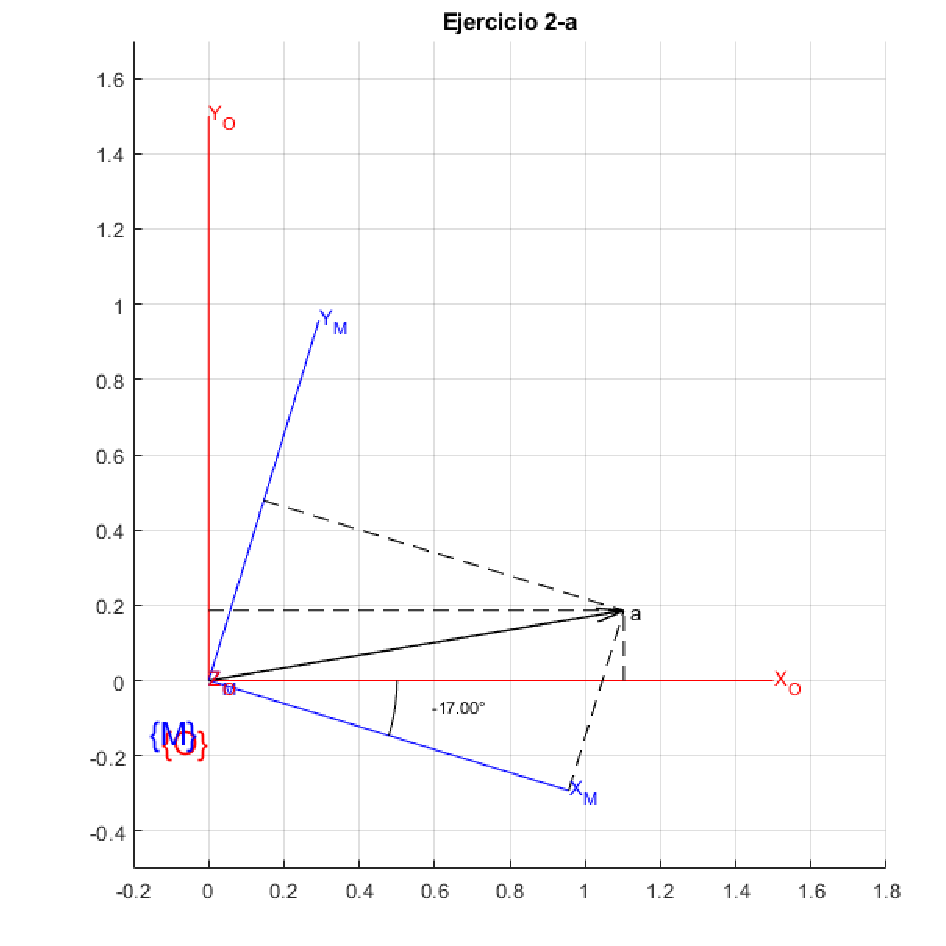
\includegraphics{4-Ejercicio_2_a.pdf}}
    \end{adjustbox}
    \caption{Sistemas M y O superpuestos - Vector con guías de proyección y cota de ángulo}
\end{figure}

\subsection{Inciso b}
\begin{equation*}
    \prescript{M}{}{b} = 
    \begin{bmatrix}
        0 & 0 & 1
    \end{bmatrix}
    \rightarrow \{M\} \, \text{rotó} \,  35^\circ \, \text{en}\, X_O
\end{equation*}

\begin{equation*}
    \prescript{O}{}{b} = 
    \begin{bmatrix}
        0 & -0.5736 & 0.8192
    \end{bmatrix}
\end{equation*}

\begin{figure}[H]
    \centering
    \begin{adjustbox}{scale = 0.85, max width=\columnwidth}
        \framebox{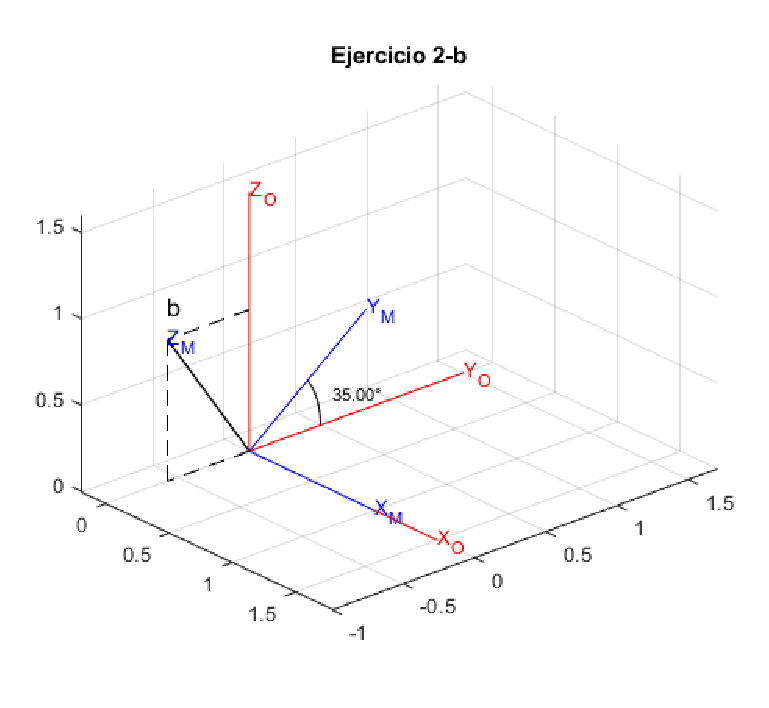
\includegraphics{5-Ejercicio_2_b.pdf}}
    \end{adjustbox}
    \caption{Sistemas M y O superpuestos - Vector con guías de proyección y cota de ángulo}
\end{figure}

\subsection{Inciso c}
\begin{equation*}
    \prescript{M}{}{c} = 
    \begin{bmatrix}
        1 & 0.5 & 0.3
    \end{bmatrix}
    \rightarrow \{M\} \, \text{rotó} \,  90^\circ \, \text{en}\, Y_O
\end{equation*}

\begin{equation*}
    \prescript{O}{}{c} = 
    \begin{bmatrix}
        0.3 & 0.5 & -1
    \end{bmatrix}
\end{equation*}

\begin{figure}[H]
    \centering
    \begin{adjustbox}{scale = 0.85, max width=\columnwidth}
        \framebox{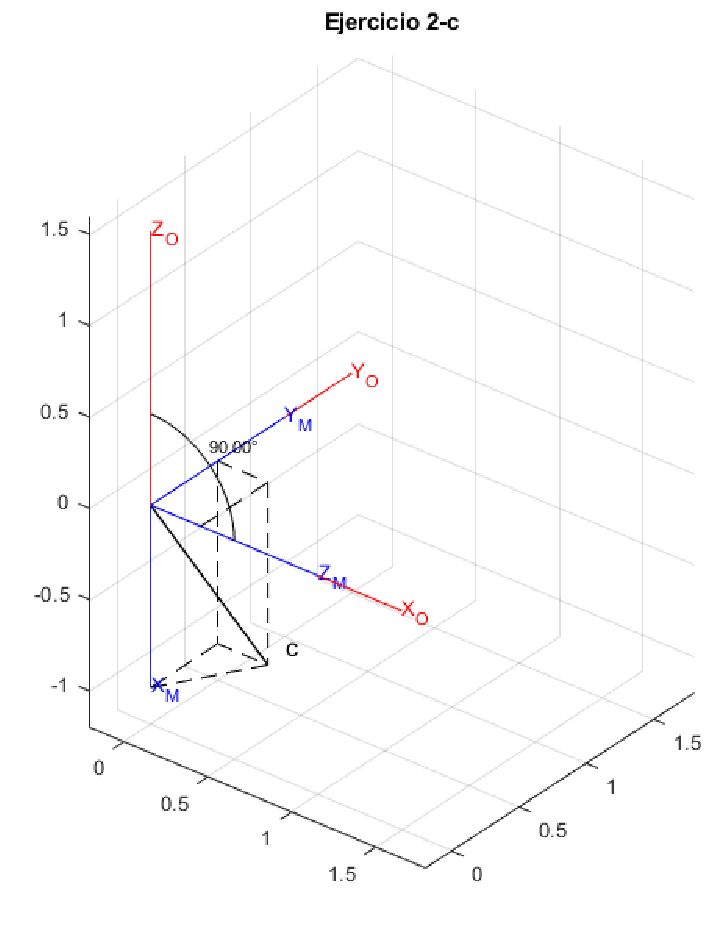
\includegraphics{6-Ejercicio_2_c.pdf}}
    \end{adjustbox}
    \caption{Sistemas M y O superpuestos - Vector con guías de proyección y cota de ángulo}
\end{figure}

\section{Ejercicio 3}
Escriba en forma general las matrices de transformación homogénea que
representan los siguientes casos:

\subsection{a. Traslación pura en el espacio}

Traslación a un punto $\mathbf{p}$ de coordenadas $\mathbf{\left[x\,y\,z\right]}$ en el sistema \textbf{\{O\}}.
\begin{equation*}
    \prescript{O}{}{T_M} = Tras(p) = 
    \begin{bmatrix}
        1 & 0 & 0 & x \\
        0 & 1 & 0 & y \\
        0 & 0 & 1 & z \\
        0 & 0 & 0 & 1
    \end{bmatrix}
\end{equation*}

\subsection{b. Rotación en el eje X}

Rotación de un ángulo $\mathbf{\alpha}$ (roll) respecto del eje X.
\begin{equation*}
    \prescript{O}{}{T_M} = Rot\left(\alpha, X\right) = 
    \begin{bmatrix}
        1 & 0            & 0             & 0 \\
        0 & \cos(\alpha) & -\sin(\alpha) & 0 \\
        0 & \sin(\alpha) & \cos(\alpha)  & 0 \\
        0 & 0            & 0             & 1
    \end{bmatrix}
\end{equation*}

\subsection{c. Rotación en el eje Y}

Rotación de un ángulo $\mathbf{\beta}$ (pitch) respecto del eje Y.
\begin{equation*}
    \prescript{O}{}{T_M} = Rot\left(\beta, Y\right) = 
    \begin{bmatrix}
        \cos(\beta) & 0            & -\sin(\beta)   & 0 \\
        0           & 1            & 0              & 0 \\
        \sin(\beta) & 0            & \cos(\beta)    & 0 \\
        0           & 0            & 0              & 1
    \end{bmatrix}
\end{equation*}

\subsection{d. Rotación en el eje Z}

Rotación de un ángulo $\mathbf{\gamma}$ (yaw) respecto del eje Z.
\begin{equation*}
    \prescript{O}{}{T_M} = Rot\left(\gamma, Z\right) = 
    \begin{bmatrix}
        \cos(\gamma) & -\sin(\gamma) & 0 & 0 \\
        \sin(\gamma) & \cos(\gamma)  & 0 & 0 \\
        0            & 0             & 1 & 0 \\
        0            & 0             & 0 & 1
    \end{bmatrix}
\end{equation*}

\section{Ejercicio 4 (obligatorio)}
En la siguiente figura se observa el vector $\mathbf{\alpha}$ respecto del sistema $\mathbf{\{M\}}$.
El punto $\mathbf{M}$ respecto de $\mathbf{\{O\}}$ es $\prescript{O}{}{p_M} = \left(7,4\right) $.

\begin{figure}[H]
    \centering
    \begin{adjustbox}{scale = 0.85, max width=\columnwidth}
        \framebox{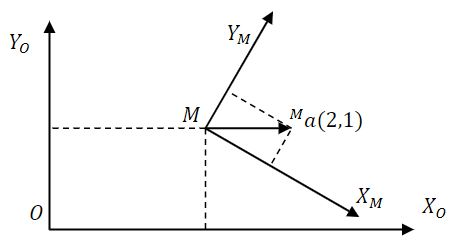
\includegraphics{7-Ejercicio_4.JPG}}
    \end{adjustbox}
    \caption{Gráfica del enunciado.}
\end{figure}

\subsection{Inciso a.}
\textbf{Halle, por el método que elija, el ángulo de rotación del sistema {M} respecto de {O}.}
\vspace{0.5 cm}

Como el vector $a$ es paralelo a $\mathbf{X_O}$, 
el ángulo que forma con $\mathbf{X_M}$ (sentido dextrógiro)
es el ángulo que se debe rotar este eje para que sea paralelo a $\mathbf{X_O}$
, es decir, el ángulo de la transformación inversa de rotación y el opuesto del 
ángulo que buscamos.

Ese ángulo se determina utilizando la función $\mathbf{atan2}$ de MATLAB tomando las coordenadas
de $a$ en el sistema $\mathbf{\{M\}}$ y luego obteniendo el ángulo opuesto.

\[
    \gamma \text(yaw) = -26.56^\circ
\]

\subsection{Inciso b.}
\textbf{Exprese la matriz de transformación homogénea que describe la posición y orientación
del sistema \{M\} respecto de \{O\}.}
\vspace{0.5 cm}

Se usa \textbf{trotz} para obtener la matriz de rotación.

\begin{equation*}
    \prescript{O}{}{T_M} = 
    \begin{bmatrix}
        0.8944  & 0.4472       & 7 \\
        -0.4472 & 0.8944       & 4 \\
        0       & 0            & 1
    \end{bmatrix}
\end{equation*}

\subsection{Inciso c.}
\textbf{Use la transformación hallada para representar el vector $a$ respecto del sistema \{O\}.
Verifique gráficamente el resultado.}
\vspace{0.5 cm}

Se obtiene segun \cref{transformacion}
\[
    \prescript{O}{}{a} =
    \begin{bmatrix}
        9.24\\
        4.00
    \end{bmatrix}
\]

\begin{figure}[H]
    \centering
    \begin{adjustbox}{scale = 0.85, max width=\columnwidth}
        \framebox{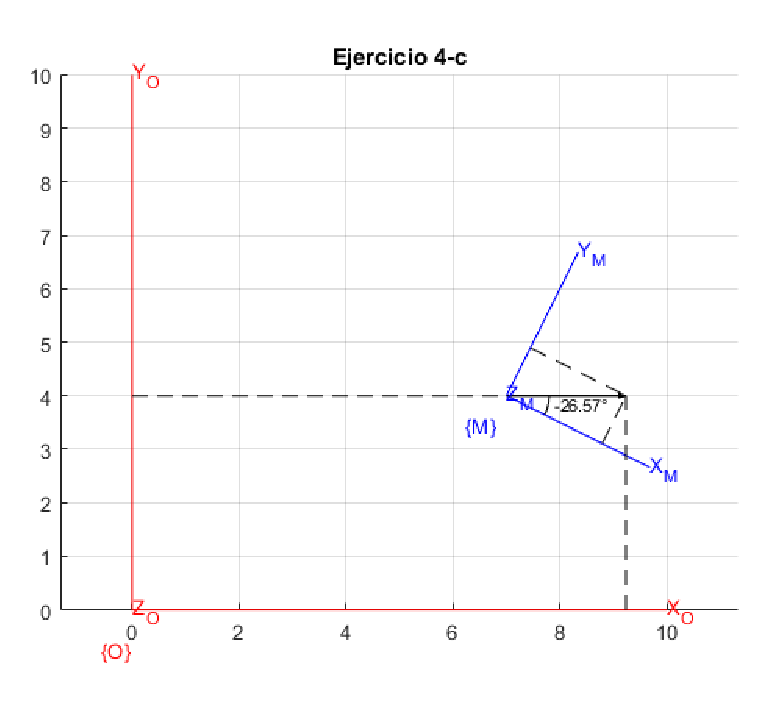
\includegraphics{8-Ejercicio_4_c.pdf}}
    \end{adjustbox}
    \caption{Verificación gráfica del ejercicio.}
\end{figure}

\section{Ejercicio 5}
Escriba la matriz de transformación homogénea que representa la posición y
orientación del sistema \{M\} respecto de \{O\} para cada caso. Realice un gráfico donde se
aprecie la diferencia.

\subsection{Inciso a.}
\textbf{El sistema {M} giró 45° respecto del eje $Y_O$, luego se trasladó un vector $\prescript{M}{}{p} = (0, 0, 1)$}
\vspace{0.5 cm}

Se usa \textbf{troty} con $\beta = 45^\circ$ y se obtiene la matriz de trasnformación homogénea R.
Luego se usa \textbf{transl} con $\prescript{M}{}{p}$ y se obtiene la matriz de transformación homogénea T.
Se obtiene $\prescript{O}{}{T_M} = R*T$.

\subsection{Inciso b.}
\textbf{El sistema {M} se trasladó un vector  $\prescript{O}{}{p}$ = (0, 0, 1), luego giró 45° respecto del eje $Y_M$.}
\vspace{0.5 cm}

Se usa \textbf{transl} con $\prescript{O}{}{p}$ y se obtiene la matriz de transformación homogénea T.
Luego se usa \textbf{troty} con $\beta = 45^\circ$ y se obtiene la matriz de trasnformación homogénea R.
Se obtiene $\prescript{O}{}{T_M} = T*R$.

\begin{figure}[H]
    \centering
    \begin{adjustbox}{scale = 0.85, max width=\columnwidth}
        \framebox{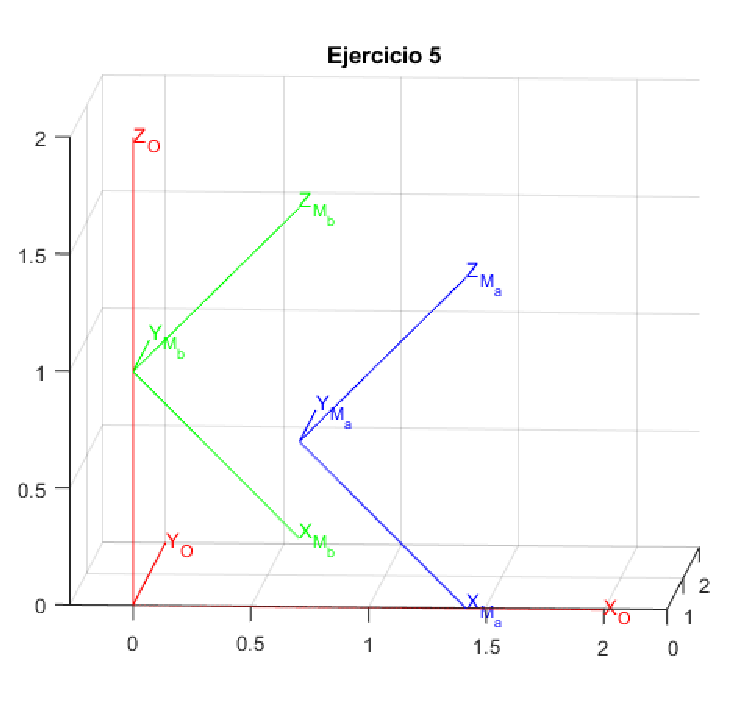
\includegraphics{9-Ejercicio_5.pdf}}
    \end{adjustbox}
    \caption{Diferencia entre los sistemas de referencia obtenidos.}
\end{figure}

\section{Ejercicio 6}
Exprese el vector $\prescript{O}{}{p}$ = (0.5, 0, 1) respecto del sistema \{M\} de cada caso del
ejercicio anterior.

De \cref{transformacion} se puede obtener:

\begin{equation}
    \prescript{M}{}{a} = \prescript{O}{}{T_M}^{-1}\prescript{O}{}{a}
    \label{transformacion inversa}
\end{equation}

\begin{equation}
    \prescript{O}{}{T_M}^{-1} =
    \begin{bmatrix}
        R^T & -R^T\prescript{O}{}{p_M}\\
        0   &   1
    \end{bmatrix}
    \label{matriz homogenea inversa}
\end{equation}

Sin embargo obtendremos la solución de los problemas utilizando el operador ''\textbackslash'' de MATLAB.

\subsection{Inciso a}
\[
    \prescript{O}{}{p} =
    \begin{bmatrix}
        -0.3536\\
        0      \\
        0.0607
    \end{bmatrix}
\]
\subsection{Inciso b}
\[
    \prescript{O}{}{p} =
    \begin{bmatrix}
        0.3536\\
        0     \\
        0.3536
    \end{bmatrix}
\]

\section{Ejercicio 7.}
Analizar la siguiente transformación compuesta e indicar V o F. Considere que $T$
representa la posición y orientación de un sistema de referencia \{M\} respecto de otro sistema
de referencia \{O\}.

\[T = TrotX(\alpha) Ttrans(0,2,0) TrotY(\beta)\]

\subsection{Inciso a}
\textbf{El sistema \{M\} sufrió una rotación $\alpha$ respecto de $X_O$, luego una traslación de 2
unidades sobre el eje $Y_O$, y finalmente una rotación $\beta$ respecto de este mismo eje.}
\vspace*{0.5 cm}

\textbf{V}. Si consideramos que el sistema sistema obtenido en las transformaciones intermedias
conserva el nombre \{O\} y solamente se denomina \{M\} al sistema obtenido luego de todas las transformaciones realizadas.

\subsection{Inciso b}
\textbf{El sistema {M} sufrió una rotación $\alpha$ respecto de $X_M$, luego una traslación de 2
unidades sobre el eje $Y_M$, y finalmente una rotación $\beta$ respecto de este mismo eje}
\vspace*{0.5 cm}

\textbf{F}. Las transformaciones deberían ir con el sub-índice O.

\subsection{Inciso c}
\textbf{Un vector $p$ expresado en \{O\} puede expresarse en \{M\} realizando el producto: $\prescript{M}{}{p} =
T. p$}
\vspace*{0.5 cm}

\textbf{F}. La premultiplicación debería ser por la inversa T.

\subsection{Inciso d}
\textbf{Un vector $p$ expresado en \{M\} puede expresarse en \{O\} realizando el producto: $\prescript{O}{}{p} =
T. p$}
\vspace*{0.5 cm}

\textbf{V}.

\section{Ejercicio 8}
En función de las siguientes matrices escritas en forma simbólica halle la expresión
correcta para cada caso:

\begin{itemize}
    \item $\prescript{O}{}{T_M}$: matriz de trasformación homogénea del sistema \{M\} respecto de \{O\}.
    \item $\prescript{M}{}{T_A}$: matriz de trasformación homogénea del sistema \{A\} respecto de \{M\}.
    \item $\prescript{A}{}{T_B}$: matriz de trasformación homogénea del sistema \{B\} respecto de \{A\}.
    \item $\prescript{O}{}{T_F}$: matriz de trasformación homogénea del sistema \{F\} respecto de \{O\}.
    \item $\prescript{F}{}{T_D}$: matriz de trasformación homogénea del sistema \{D\} respecto de \{F\}.
\end{itemize}

\subsection{\{B\} respecto de \{O\}}
\[\prescript{O}{}{T_B} = \prescript{O}{}{T_M} \prescript{M}{}{T_A} \prescript{A}{}{T_B}\]

\subsection{\{F\} respecto de \{B\}}
\[\prescript{B}{}{T_F} = \prescript{O}{}{T_B}^{-1} \prescript{O}{}{T_F}\]

\subsection{\{B\} respecto de \{D\}}
\[\prescript{D}{}{T_B} = \prescript{F}{}{T_D}^{-1} \prescript{B}{}{T_F}^{-1} \]

\end{document}